\documentclass[man,a4paper,noextraspace,apacite]{apa6}\usepackage[]{graphicx}\usepackage[]{color}
%% maxwidth is the original width if it is less than linewidth
%% otherwise use linewidth (to make sure the graphics do not exceed the margin)
\makeatletter
\def\maxwidth{ %
  \ifdim\Gin@nat@width>\linewidth
    \linewidth
  \else
    \Gin@nat@width
  \fi
}
\makeatother

\definecolor{fgcolor}{rgb}{0.345, 0.345, 0.345}
\newcommand{\hlnum}[1]{\textcolor[rgb]{0.686,0.059,0.569}{#1}}%
\newcommand{\hlstr}[1]{\textcolor[rgb]{0.192,0.494,0.8}{#1}}%
\newcommand{\hlcom}[1]{\textcolor[rgb]{0.678,0.584,0.686}{\textit{#1}}}%
\newcommand{\hlopt}[1]{\textcolor[rgb]{0,0,0}{#1}}%
\newcommand{\hlstd}[1]{\textcolor[rgb]{0.345,0.345,0.345}{#1}}%
\newcommand{\hlkwa}[1]{\textcolor[rgb]{0.161,0.373,0.58}{\textbf{#1}}}%
\newcommand{\hlkwb}[1]{\textcolor[rgb]{0.69,0.353,0.396}{#1}}%
\newcommand{\hlkwc}[1]{\textcolor[rgb]{0.333,0.667,0.333}{#1}}%
\newcommand{\hlkwd}[1]{\textcolor[rgb]{0.737,0.353,0.396}{\textbf{#1}}}%

\usepackage{framed}
\makeatletter
\newenvironment{kframe}{%
 \def\at@end@of@kframe{}%
 \ifinner\ifhmode%
  \def\at@end@of@kframe{\end{minipage}}%
  \begin{minipage}{\columnwidth}%
 \fi\fi%
 \def\FrameCommand##1{\hskip\@totalleftmargin \hskip-\fboxsep
 \colorbox{shadecolor}{##1}\hskip-\fboxsep
     % There is no \\@totalrightmargin, so:
     \hskip-\linewidth \hskip-\@totalleftmargin \hskip\columnwidth}%
 \MakeFramed {\advance\hsize-\width
   \@totalleftmargin\z@ \linewidth\hsize
   \@setminipage}}%
 {\par\unskip\endMakeFramed%
 \at@end@of@kframe}
\makeatother

\definecolor{shadecolor}{rgb}{.97, .97, .97}
\definecolor{messagecolor}{rgb}{0, 0, 0}
\definecolor{warningcolor}{rgb}{1, 0, 1}
\definecolor{errorcolor}{rgb}{1, 0, 0}
\newenvironment{knitrout}{}{} % an empty environment to be redefined in TeX

\usepackage{alltt}
\usepackage{apacite}
\title{What Does Perspective Taking Do for Empathy?}
\shorttitle{Perspective Taking}
\author{Joshua D. Wondra}
\affiliation{University of Michigan}

\abstract{Abstract TBD}
\keywords{empathy, vicarious emotions, perspective taking}

\authornote{Joshua D. Wondra, Department of Psychology, University of Michigan.

Correspondence concerning this article should be addressed to Josh Wondra, Department of Psychology, University of Michigan, 530 Church St., Ann Arbor, MI 48109-1043.dh

Contact: jdwondra@umich.edu}
\IfFileExists{upquote.sty}{\usepackage{upquote}}{}
\begin{document}

\maketitle

When someone is going through an emotional experience, people are often advised to take that person's perspective so that they will understand and feel how that person feels. Psychologists, too, believe in this power of perspective taking---many experiments use it to get subjects to empathize \cite<e.g., >{Batson1997, Lamm2007}. But does perspective taking make people feel the specific emotions that another person feels?

When it comes to answering this question, existing research is surprisingly limited. There are two reasons for this. First, in most studies the target of perspective taking feels sad, distressed, or anxious, all of which involve appraisals that the situation is or might be out of one's control \cite{Smith1985, Ellsworth1988}. This means that perspective taking might uniquely affect emotions that are felt in uncontrollable circumstances. Specifically, perspective taking decreases actor-observer bias, which involves the tendency to make more dispositional attributions for others and situational attributions for oneself \cite{Galper1976, Storms1973}. Perhaps perspective taking increases empathy with emotions that involve appraisals that situational factors are in control, such as sadness, but not empathy with emotions that involve appraisals that some human agent is in control, such as anger.

The second limit of existing research is the comparison condition to perspective taking, which is most commonly to tell subjects to remain objective and detached \cite{McAuliffe2016}. The problem is that these instructions are not a neutral control condition. Instead, they tell subjects to down-regulate their vicarious emotions, which makes it unclear if the observed effects are due to increased empathy from perspective taking, decreased empathy from remaining objective, or both.

In this study, I addressed the first limitation of existing research by exposing subjects to someone who felt either sad or angry about a misfortune, and the second limitation by including a neutral control condition. I tested three hypotheses.

\begin{enumerate}
  \item Perspective taking increases empathy with specific emotions. If so, then subjects who are instructed to take a target's perspective should feel sadder when the target is sad and angrier when the target is angry compared to subjects who received no instructions. 
  \item Perspective taking only increase empathy with emotions that involve appraisals that situational factors are in control. If so, then subjects who are instructed to take a target's perspective should feel sadder when the target is sad when they are instructed to take her perspective compared to subjects who received no instructions. There should be no effect of perspective taking on subjects' emotions when the target is angry.
  \item Remaining objective decreases empathy. If so, then subjects who are instructed to remain objective should feel less sad and angry compared to subjects who receive no instructions.
\end{enumerate}

I also tested the effects of perspective taking and remaining objective on sympathy.

\section{Method}



\subsection{Overview}

    Subjects read a bogus letter from someone else who described an experience that made her feel sad or angry. Subjects were instructed to take the other person's perspective, to remain objective, or they received no instructions. The study had a 2 (Emotion: sad, angry) x 3 (Instructions: perspective taking, objective, control) between-subjects factorial design. Subjects reported their own emotions and appraisals of the letter writer's situation and their perceptions of the letter writer's emotions and appraisals.
    
\subsection{Subjects}

    Subjects were 404 (239 women, 161 men, one transgender, three did not report gender) undergraduate students and community members who participated for course credit or \$5. Data from an additional 39 subjects were excluded; 20 subjects suspected that the letter they read was not real, 13 were inattentive, four were non-native English speakers, one reported that he had a concussion, and one learned which experimental condition he was in due to experimenter error. Subjects' ages ranged from 18 to 64 (Median = 19).

\subsection{Procedure}
Subjects participated individually. They were told that the researchers were studying how people communicate about personal experiences and react to others' personal experiences. They were told that they would begin by writing about a personal experience to a future participant and then they would read about the personal experience of someone else who participated in the study earlier in the semester. The letter exchange and perspective taking instructions in this study are similar to the procedure used by Batson and colleagues \cite<e.g., >{Batson2002, Batson2007a, Batson2007b}, except that subjects also wrote a letter to better sell the cover story.

Subjects received a pen, a piece of paper, and an envelope. They were told to write a letter to a future participant and then put their letter in the envelope. They were asked to write one or two paragraphs about something interesting that happened to them recently. 

Next, the experimenter told subjects that they would read a letter that was randomly selected from someone who participated earlier in the semester. Then they would complete a questionnaire on the computer about their reactions to the letter. Subjects in the perspective taking and objective conditions were told that the way they read the letter was important. Those in the perspective taking condition were told to ``try to imagine how the other person feels about what is described. Try to imagine how it has affected her life and how she feels as a result,'' whereas those in the objective condition were told to ``try not to get caught up in how the other person feels; just remain objective and detached''. Subjects in the control condition received no instructions.

Subjects read the letter from Melissa, who was upset about missing her best friend's bachelorette party in New York City due to car problems. Subjects were randomly assigned to read a letter where the car problems were due to bad circumstances and Melissa felt sad, or where the car problems were her friend's fault and Melissa felt angry. The sad (\textit{angry}) letter read:

\begin{quote}
Dear future participant,

    So I'm supposed to write about something interesting that happened to me recently. Well, a couple of weeks ago I tried to go on a road trip with a friend, but couldn't go because of bad circumstances \textit{(because of my friend who was supposed to drive)}. My best friend of 10 years is getting married in two months and she asked me to be her maid of honor, so of course I got to plan her bachelorette party. We always wanted to visit New York City together so that was the perfect place for us to do it. One of my friends here wanted to visit his friends in NYC that weekend so he offered to drive us both. He was having some car troubles so I asked if he would be able to get it fixed before the trip or if I should try to find another way to get there. He told me that he took the car in for repairs and we were all set, so we left a few days later. Then suddenly, when we were a quarter of the way there, his car started making noises and it just died. So it turns out that he got the car fixed but the replacement part was defective \textit{(he didn't get the car fixed and he had lied to me about taking it in)}. We towed the car to a mechanic but they didn't have the parts they needed to fix the car. So I called another friend to come pick me up and take me back to Ann Arbor. There weren't any more flights to NYC so I got stuck here and missed my best friend's bachelorette party. I cried about it for a few days after we got back and I'm tearing up thinking about it now \textit{(I didn't talk to my friend for a few days after we got back and I'm fuming thinking about it now)}. I still can't believe that happened and I'm still really upset about it.

Sincerely,

Melissa

\end{quote}

After subjects read the letter, they completed a questionnaire on the computer about their emotions and appraisals.

First, subjects reported their main feelings after reading the letter in an open-ended format.


Second, subjects reported how much they felt several specific emotions that appeared in a randomized order on a 5-point Likert-type scale (1 = Not at all, 5 = Extremely). The items ``sad'' and ``down'' were averaged to measure sadness (\textit{r} = 0.62), ``angry'' and ``mad'' were averaged to measure anger (/textit{r} = 0.84), and ``sympathetic'' and ``compassionate'' were averaged to measure sympathy (\textit{r} = 0.51). The rest of the emotions were filler items.

Third, subjects reported their perceptions of the letter writer's main feelings in open-eneded and closed-ended formats that paralleled the reports of their own emotions, but without the items ``sympathetic'' and ``compassionate''. These were included to explore how perspective taking affected empathy, if there was evidence of an effect.

Fourth, subjects reported their appraisals of the experience the letter writer described. The questions measured appraisals of pleasantness ("How unpleasant was it?"), self-agency and control ("How much do you feel like you are responsible for what happened?", "How much do you feel like you had the power to do something about the situation?"), the letter writer's agency and control ("How much do you feel that the other participant is responsible for what happened?", "How much do you feel that the other participant had the power to do something about the situation?"), other-agency and control ("How much do you feel that someone aside from the other participant is responsible for what happened?", "How much do you feel that someone aside from the other participant had the power to do something about the situation?"), situational agency and control ("How much do you feel that circumstances beyond anyone's control are responsible for what happened?", "How much do you feel that the situation was caused by a combination of many factors?", "How much do you feel that no one had the power to do anything about the situation?", "How much do you feel that the situation was out of anyone's control?"), and legitimacy ("To what extent was what happened morally wrong?"). Each question had a 5-point Likert-type response scale (1 = Not at all, 5 = Extremely). These were also included to explore how perspective taking affected empathy, if there was evidence of an effect.

Finally, subjects completed a parallel questionnaire that measured their perceptions of the letter writer's appraisals and they completed the Interpersonal Reactivity Index \cite{Davis1980, Davis1983}. Both of these were included for exploratory purposes and are not discussed further.

After completing the questionnaire, subjects were debriefed and thanked for their participation. 

\section{Results}



\subsubsection{Coding the Open-Ended Emotion Reports} To analyze subjects' open-ended reports of emotions, groups of emotion words were created that seemed to communicate similar feelings. Subjects' experimental conditions were removed from their open-ended responses. All of the words that subjects used in the emotion reports were identified. Then the words that communicated similar feelings were grouped together. Each subject received a score of 1 if they mentioned at least one word in the emotion group and a score of 0 if they did not. For the present study, I only analyzed sadness, anger, and sympathy. Table 1 displays the words that were placed in these groups. 

\begin{table}
Table 1

\textit{Subjects' open-ended reports of their own emotions.}

\begin{tabular}{l c}
    \hline
    Emotion Group & Emotion Words \\
    \hline
    Sadness & defeat, depressed, depression, despair, disappointed, disappointing, \\
    & disappointment, disheartened, down, heartbroken, helpless, helplessness, \\
    & hopeless, let down, melancholy, sad, saddened, sadness, \\
    & solemn, sorrow, want to cry \\
    & \\
    Anger & aggravation, agitated, anger, angry, annoyance, annoyed, \\ 
    & bitter, furious, indignance, irritation, mad, outraged, pissed \\
    & \\
    Sympathy & apologetic, caring, compassion, compassionate, concern, concerned, \\
    & consoling, empathetic, empathic, empathy, pity, sorriness, \\ 
    & sorry, sympathetic, sympathy, wish I could help \\
    \hline
\end{tabular}
\end{table}

I used logistic regression to find the predicted probability that a subject listed an emotion group. To test the main hypotheses, we used contrasts to compare the three perspective taking conditions within each emotion group. 

\subsubsection{Testing the Hypotheses} The hypotheses about the effects of perspective taking and remaining objective on vicarious emotions were tested using planned contrasts. The contrasts tested for differences in the perspective conditions within each emotion condition separately. To test for differences in the probability that subjects reported feeling sad, angry, or sympathetic in their open-ended responses, I tested separate logistic regression models with one of the planned contrasts entered as a predictor along with the rest of the orthogonal contrasts that were needed to complete the experimental design. 


\subsection{Did Perspective Taking Make Subjects Feel How Melissa Felt, or Did it Only Make Them Feel Sad?}

If perspective taking makes people feel the same emotions that others feel, then subjects who took Melissa's perspective should have felt sadder when Melissa felt sad and angrier when Melissa felt angry than subjects who were in the control condition. If, on the other hand, perspective taking only makes people feel vicarious emotions that involve appraisals that the situation is uncontrollable, then subjects who took Melissa's perspective should have felt sadder when Melissa felt sad, but not angrier when Melissa felt angry.

\subsubsection{Open-ended data}

\begin{figure}
\begin{knitrout}
\definecolor{shadecolor}{rgb}{0.969, 0.969, 0.969}\color{fgcolor}
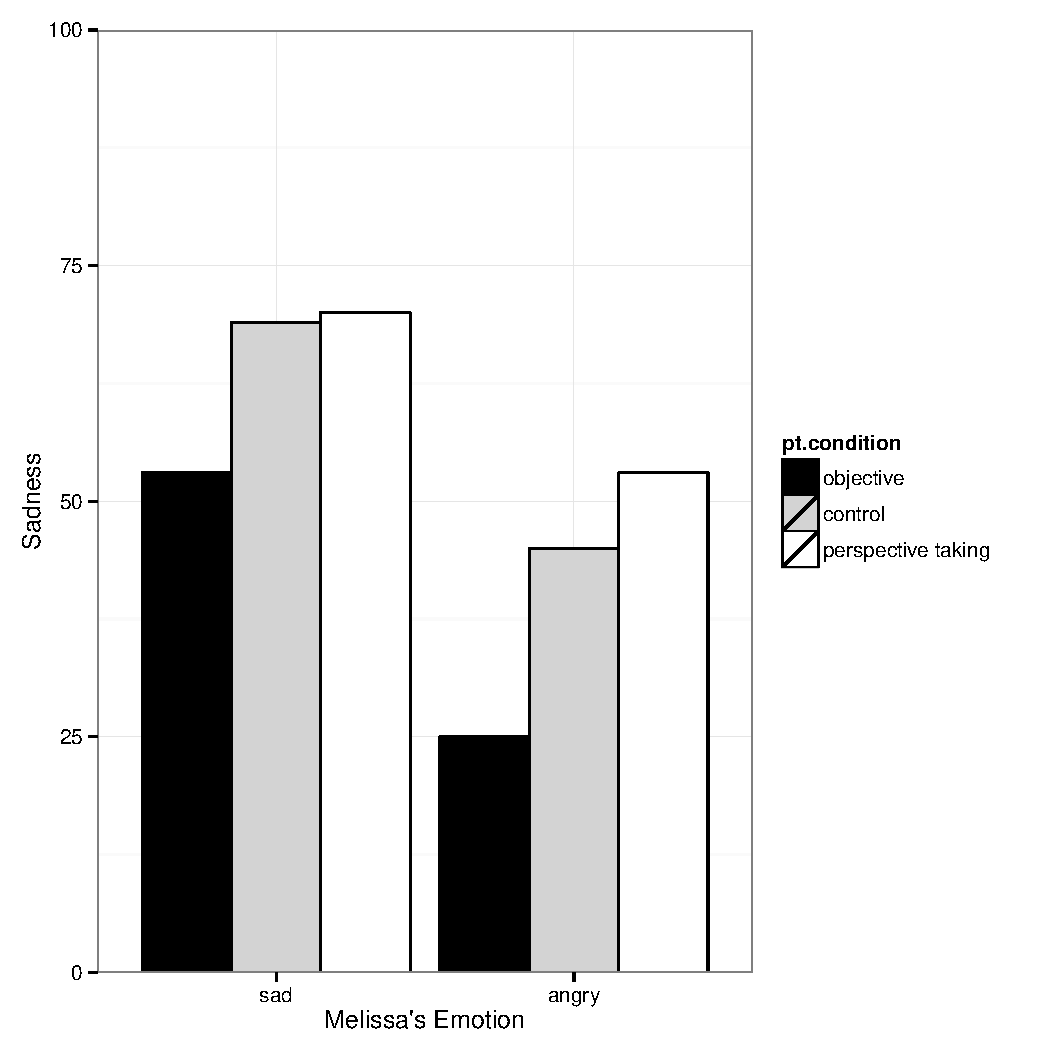
\includegraphics[width=\maxwidth]{figure/Figure1Sad-1} 

\end{knitrout}
\textit{Figure 1. Probability that subjects reported feeling sad by condition.}
\end{figure}


\begin{figure}
\begin{knitrout}
\definecolor{shadecolor}{rgb}{0.969, 0.969, 0.969}\color{fgcolor}
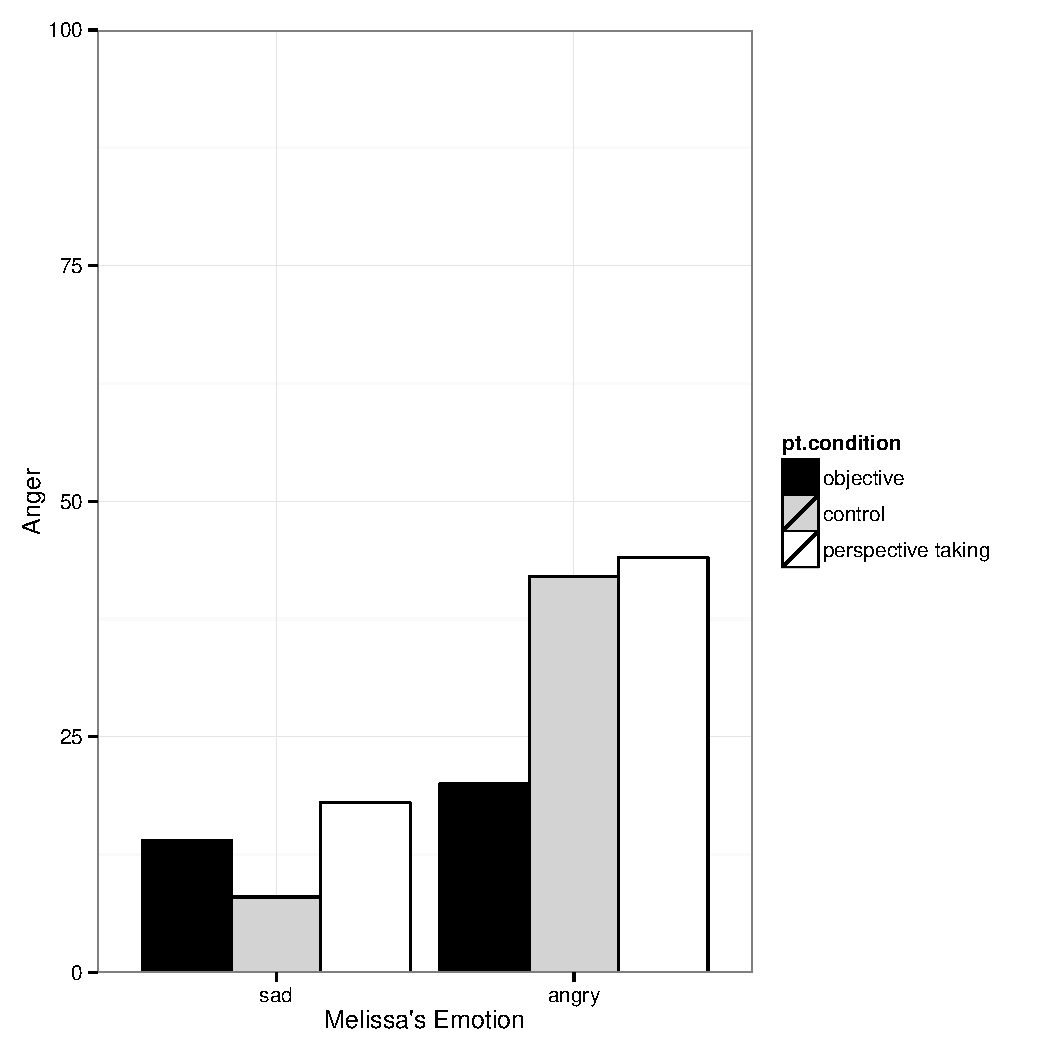
\includegraphics[width=\maxwidth]{figure/Figure2Angry-1} 

\end{knitrout}
\textit{Figure 2. Probability that subjects reported feeling angry by condition.}
\end{figure}



Figure 1 displays the probability that subjects reported feeling sad by condition and Figure 2 displays the probability that subjects reported feeling angry by condition. When Melissa was sad, subjects were just as likely to feel sad when they took her perspective (70\%) as when they received no instructions (69\%), \textit{B} = 0.03, \textit{SE} = 0.19, \textit{Z} = 0.14, \textit{p} = 0.88, 95\% CI [\ensuremath{-0.34}, 0.39]. Similarly, when Melissa was angry, subjects were just as likely to report feeling angry when they took her perspective (44\%) as when they received no instructions (42\%), \textit{B} = 0.04, \textit{SE} = 0.17, \textit{Z} = 0.22, \textit{p} = 0.82, 95\% CI [\ensuremath{-0.3}, 0.38]. There was no evidence that perspective taking had an effect on subjects' vicarious emotions.

\subsubsection{Closed-ended data}

\begin{figure}
\begin{knitrout}
\definecolor{shadecolor}{rgb}{0.969, 0.969, 0.969}\color{fgcolor}
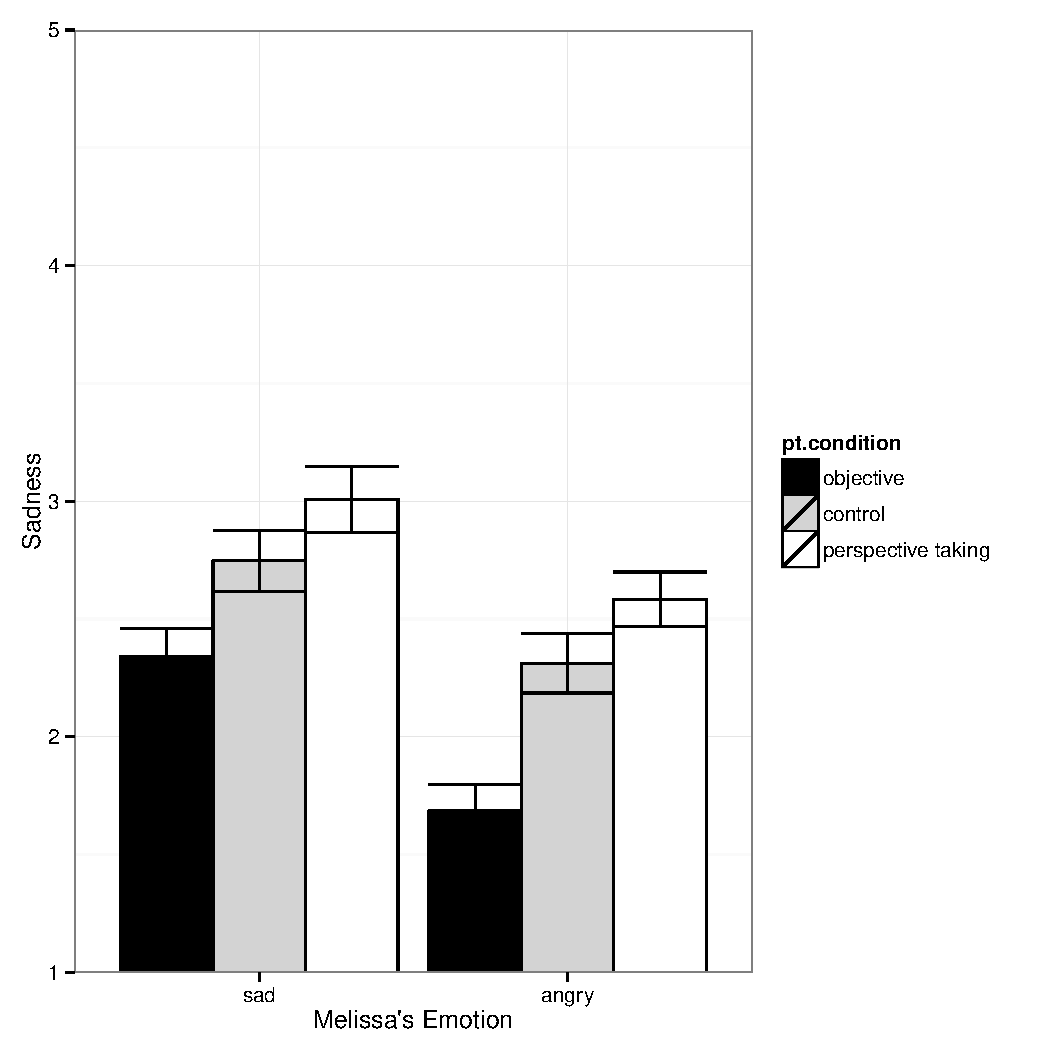
\includegraphics[width=\maxwidth]{figure/Figure3Sad-1} 

\end{knitrout}
\textit{Figure 3. Subjects' average sadness by condition. The bars represent standard errors.}
\end{figure}


\begin{figure}
\begin{knitrout}
\definecolor{shadecolor}{rgb}{0.969, 0.969, 0.969}\color{fgcolor}
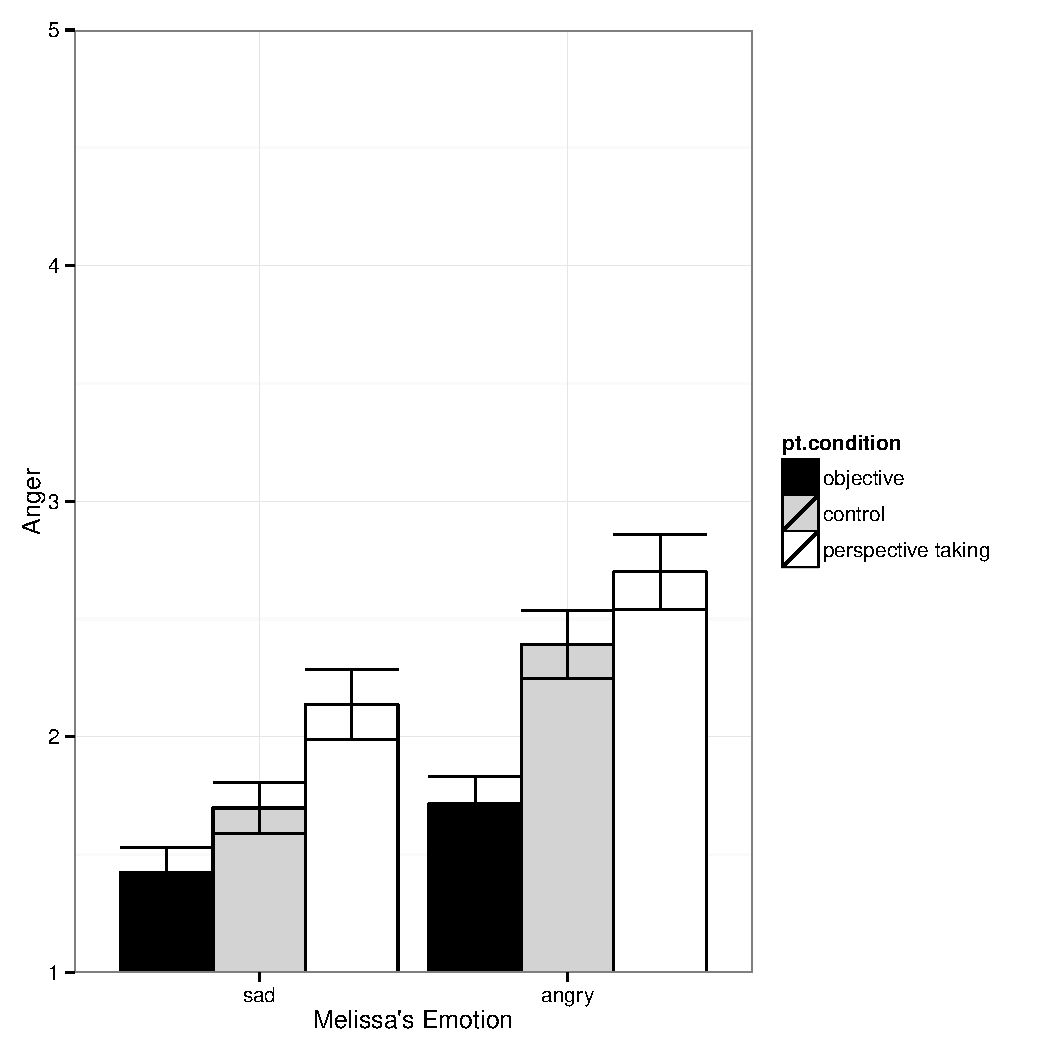
\includegraphics[width=\maxwidth]{figure/Figure4Angry-1} 

\end{knitrout}
\textit{Figure 4. Subjects' average anger by condition. The bars represent standard errors.}
\end{figure}



Figure 3 displays subjects' average sadness by condition and Figure 4 displays subjects' average anger by condition. When Melissa was sad, subjects felt as sad when they took her perspective (\textit{M} = 3.01, \textit{SD} = 1.14) as when they received no instructions (\textit{M} = 2.75, \textit{SD} = 1.1), \textit{t}(398) = 1.5, \textit{p} = 0.13, 95\% CI [\ensuremath{-0.04}, 0.3]. When Melissa was angry, there was a non-significant trend for subjects to feel angrier when they took her perspective (\textit{M} = 2.7, \textit{SD} = 1.28) than when they received no instructions (\textit{M} = 2.39, \textit{SD} = 1.2), \textit{t}(396) = 1.66, \textit{p} = 0.098, 95\% CI [\ensuremath{-0.03}, 0.34]. Once again, there was little evidence that perspective taking had an appreciable effect on subjects' vicarious emotions.

\subsection{Did Perspective Taking Make Subjects Feel More Sympathetic?}

Aside from feeling how someone else feels, much research has focused on the effects of perspective taking on feeling sympathy, or empathic concern. Although perspective taking didn't make subjects feel how Melissa felt, it might have made them more sympathetic.

\subsubsection{Open-ended data}


When Melissa was sad, subjects were just as likely to feel sympathetic when they took her perspective (66\%) as when they received no instructions (68\%), \textit{B} = \ensuremath{-0.04}, \textit{SE} = 0.18, \textit{Z} = \ensuremath{-0.24}, \textit{p} = 0.81, 95\% CI [\ensuremath{-0.4}, 0.31]. Similarly, when Melissa was angry, subjects were just as likely to feel angry when they took her perspective (44\%) as when they received no instructions (42\%), \textit{B} = \ensuremath{-0.16}, \textit{SE} = 0.18, \textit{Z} = \ensuremath{-0.91}, \textit{p} = 0.36, 95\% CI [\ensuremath{-0.51}, 0.19]. There was no evidence that perspective taking made subjects feel more sympathy for Melissa.

\subsubsection{Closed-ended data}



When Melissa was sad, subjects felt as sympathetic when they took her perspective (\textit{M} = 3.69, \textit{SD} = 0.98) as when they received no instructions (\textit{M} = 3.54, \textit{SD} = 1), \textit{B} = 0.08, \textit{SE} = 0.08, \textit{t}(395) = 0.91, \textit{p} = 0.36, 95\% CI [\ensuremath{-0.09}, 0.24]. When Melissa was angry, there was a non-significant trend for subjects to feel more sympathetic when they took her perspective (\textit{M} = 3.76, \textit{SD} = 0.91) than when they received no instructions (\textit{M} = 3.43, \textit{SD} = 1.02), \textit{B} = 0.16, \textit{SE} = 0.08, \textit{t}(395) = 1.93, \textit{p} = 0.054, 95\% CI [\ensuremath{-0.003}, 0.33]. Once again, there was little evidence that perspective taking had an appreciable effect on subjects' sympathy. 

\subsection{Did Remaining Objective Make Subjects Feel Less Empathy?}

\begin{figure}
\begin{knitrout}
\definecolor{shadecolor}{rgb}{0.969, 0.969, 0.969}\color{fgcolor}
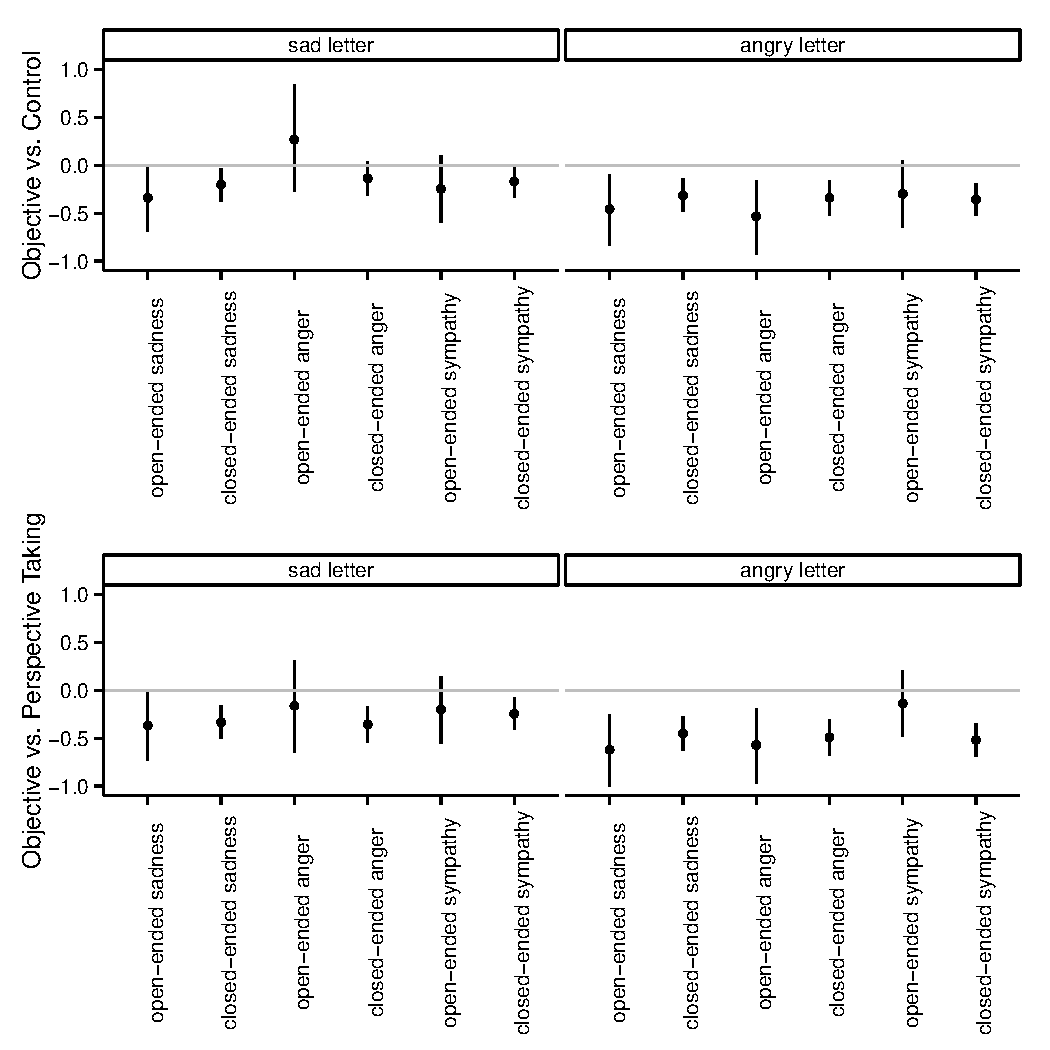
\includegraphics[width=\maxwidth]{figure/Figure5CIPlotsObjectiveVSOthers-1} 

\end{knitrout}
\textit{Figure 5. 95\% confidence intervals for the difference in subjects' emotions between the objective condition and each of the other two conditions. Negative values indicate that subjects felt weaker emotions in the objective condition than in the control and perspective taking conditions.}
\
\end{figure}

There was little evidence that perspective taking increased subjects' vicarious emotions. However, remaining objective might have decreased their vicarious emotions. Figure 5 displays 95\% confidence intervals for the difference in subjects' emotions between the objective condition and the control and perspective taking conditions. 

When Melissa was sad, subjects who remained objective did not feel as sad as those in the control and perspective taking conditions, though the comparison between the objective and control condition in the open-ended data was marginally significant (\textit{p} = .056). Subjects who remained objective also reported feeling less sympathetic than those in the other two conditions in their closed-ended responses. Although the pattern was in the same direction, there were no significant differences in subjects' open-ended reports of sympathy. 

When Melissa was angry, subjects who remained objective did not feel as angry as those in the control and perspective taking conditions. They also reported feeling less sympathetic than those in the other two conditions in their closed-ended responses, although once again this pattern was not significant in the open-ended emotion reports. 

In summary, there was strong evidence that remaining objective decrease subjects' vicarious emotions, and little evidence that perspective taking increased their vicarious emotions.


\section{Discussion}
What does perspective taking do for empathy? In the present study, it did little. Perspective taking did not increase empathy with specific emotions, nor did it increase vicarious emotions that involve appraisals that the situation is uncontrollable. Instead, when subjects were asked to remain objective they down-regulated their natural empathic reactions. These results raise two important points---one methodological, and one theoretical.

On the methodological point, researchers have used perspective taking to change prejudice and how people use stereotypes \cite{Ku2010}, perceptions of oneness and negative affect \cite{Maner2002} and, of course, empathy \cite<e.g.,>{Hawk2011, Smith1989, Toi1982}. In many studies, the alternative to perspective taking is to tell subjects to remain objective. When the research question is how empathy affects some other outcome, such as how empathy affects altruism \cite{Maner2002, Batson2002, Batson1997}, then using these two conditions as a manipulation of empathy might not be a problem. However, when the research question is how perspective taking affects some outcome, it becomes unclear whether any observed differences should be attributed to perspective taking, to remaining objective, or to both. In the present study, perspective takers felt sadder, angrier, and more sympathetic than those who remained objective. If there had been no control condition, some researchers might have thought this meant that perspective taking increases empathy, but that inference would have been dead wrong.

On the theoretical point, perspective taking should be viewed as a form of emotion regulation, but it involves the up-regulation of vicarious emotions rather than down-regulation. Consequently, effortful perspective taking only matters when the default reaction is a lack of empathy. 

In the present study, the default was to empathize, and what was effortful was to remain objective. During debriefing, the experimenters asked subjects how they tried to remain objective. Their responses sounded like the same strategies that are used in other research on emotion down-regulation \cite{Gross2015, Kross2011}. Some subjects distracted themselves from Melissa's emotions by focusing on the facts. Some subjects reappraised the letter by imagining they were reading from a novel. Others self-distanced by reminding themselves that they didn't know the person or by trying to look at the situation from an outside perspective. But regardless of the strategy, many of them also reported that it was difficult to remain objective.

Outside of the present study, sometimes the default is to feel relatively unemotional, such as when it's hard to understand the other person's emotional experience, you're motivated not to empathize \cite{Zaki2014}, or you initially appraise the other person's emotional situation as relatively neutral \cite{Wondra2015}. In these cases, remaining objective will do little because there is nothing to down-regulate. Instead, effortful perspective taking might up-regulate empathy by making you redirect attention, reprioritize your goals, or reappraise the other person's situation. 

The results of the present study suggest that learning about others' emotional experiences might be like reading a good novel or watching a good movie. If you're paying attention and you understand what's happening, you can easily get drawn in and feel for the other person. No extra effort is required, through perspective taking or otherwise.

\bibliography{ptreferences}
\bibliographystyle{apacite}

\end{document}
